\section{Verification, numerical evaluation, and reproducibility}
\label{sec:verification}

The asymptotic theorems are proved in the preceding sections. The
accompanying computations have three separate purposes: exact checks of
finite identities, certified evaluation of the proved limiting formulas,
and illustrations of finite-size convergence. None substitutes for the
proof of an asymptotic statement.

\subsection{Exact finite-field checks}
The standard-library Python program \texttt{code/verify\_exact.py} uses
integer and rational arithmetic, with an explicit implementation of
$\F_4=\F_2[z]/(z^2+z+1)$. Its recorded run passed the following checks.
\begin{center}
\begin{tabular}{@{}lr@{}}
\toprule
Identity or finite assertion & Cases\\
\midrule
Quadratic Fourier identities and polar radicals & 163\\
Plane Fourier identities on all alternating four-dimensional forms & 4,889\\
Partial Gaussian M\"obius identity & 495\\
Flag-count identity & 1,365\\
Uniform-matrix subspace moments & 2,178\\
Uniform-matrix rank-law normalization & 363\\
\bottomrule
\end{tabular}
\end{center}
The alternating-form tests exhaust all forms in dimension four over
$\F_2,\F_3,\F_4$; the quadratic tests exhaust the stated small spaces,
including nonzero pure-square forms in characteristic two. The program
also checks the truncation inequality and the nondegenerate-form count.
The exact list of parameters and scope is in
\texttt{results/exact\_checks.json}.

\subsection{Certified limiting profiles}
The program \texttt{code/compute\_profiles.py} evaluates the limiting
formulas for $q=2,3,4,5$ and $-5\le a\le5$.
Its 44 computations use 100-digit outward-rounded interval arithmetic,
400 factors for each infinite product, and the explicit Gaussian-moment
tail bound from the hidden-form section. Each saved decimal is enclosed
with absolute error at most $10^{-45}$. The dimension-tail bound in
each run is below $10^{-70}$. These are error bounds for the infinite
\emph{limit formulas}, not rates of convergence from finite $n$.

\begin{table}[htbp]
\centering\small
\begin{tabular}{@{}rrrrrr@{}}
\toprule
$q$ & $a$ & Full TV & Dimension TV & Recovery & Elimination \\
\midrule
2 & -3 & 0.14010654 & 0.05867441 & 0.14897429 & 0.00000000 \\
2 & -2 & 0.20466458 & 0.11001451 & 0.29218681 & 0.00000000 \\
2 & -1 & 0.29754118 & 0.19252540 & 0.50331096 & 0.00000000 \\
2 & 0 & 0.41149603 & 0.28878810 & 0.70156472 & 0.28878810 \\
2 & 1 & 0.64934993 & 0.28878810 & 0.83603079 & 0.57757619 \\
2 & 2 & 0.80832002 & 0.57757619 & 0.91401872 & 0.77010159 \\
2 & 3 & 0.89976122 & 0.77010159 & 0.95596960 & 0.88011610 \\
3 & 0 & 0.30597981 & 0.28006304 & 0.72406387 & 0.56012608 \\
4 & 0 & 0.24107857 & 0.22951251 & 0.77177168 & 0.68853754 \\
5 & 0 & 0.19642113 & 0.19008320 & 0.81032945 & 0.76033280 \\
\bottomrule
\end{tabular}
\caption{Selected limiting probabilities. Recovery is the optimal posterior success probability; elimination requires a one-dimensional compatible linear space. The full 44-profile table is included as CSV and JSON. Displayed digits are rounded from certified evaluations.}
\label{tab:selected-profiles}
\end{table}


\begin{figure}[htbp]
 \centering
 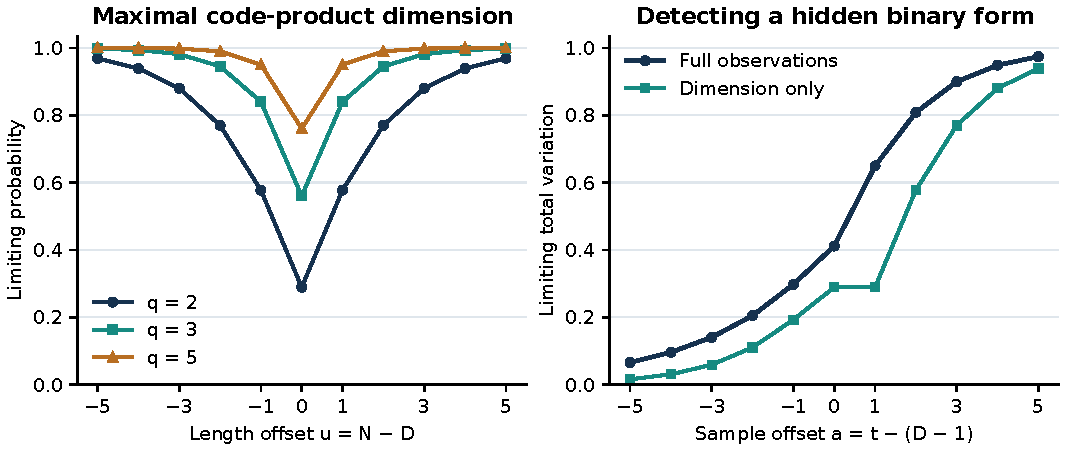
\includegraphics[width=\linewidth]{results/critical_profiles.pdf}
 \caption{Left: the limiting probability that a code product attains
 its maximal possible dimension at offset $u$ from its corrected
 dimension $D$. Right: the hidden binary-form testing limit, comparing
 full observations with the dimension statistic alone. Each plot shows
 proved formulas; the curves join discrete integer offsets.}
 \label{fig:profiles}
\end{figure}

\subsection{Finite-size illustrations}
The standard-library program \texttt{code/simulate\_binary.py} samples
actual binary square codes and actual random-plane constraints. Its
recorded run uses seed 20261127 and 1,500 trials per parameter setting,
27,000 samples in total. The output includes frequencies, Monte Carlo
standard errors, and the exact finite-size likelihood normalization for
the hidden-form experiment. Small dimensions can be far from the limit:
zero or repeated generator columns are among the finite-size effects
that disappear asymptotically. No finite-size accuracy guarantee is
inferred from these simulations.

\subsection{Proof dependency and formalization notes}
The logical route starts with Fourier separation, which gives summed
estimates for subspace inclusions. M\"obius inversion with a controlled
tail then gives universality for the entire kernel.
Quadratic character sums and low-rank counts supply the two hypotheses
for evaluations; the exact plane Fourier identity supplies them for
alternating constraints. The code applications then use an exact
adapted-basis count. For the hidden-form law, the additional ingredient
is the joint-corank theorem, whose independent ingredients are tensor
dimension surplus, mixed injection moments, and interpolation on even
nullities. The final statistical conclusions follow from an exact
likelihood and binomial size biasing.

The archive includes \texttt{FORMALIZATION\_NOTES.txt}, which identifies
these modules and their theorem statements for a future Lean development.
It is a roadmap, not an executable or checked Lean proof. The finite
checkers are executable verification of the identities they enumerate.
The LaTeX source is the complete human-readable proof.

\subsection{Rebuilding}
From the archive root, the commands are
\begin{verbatim}
python3 code/verify_exact.py
python3 code/compute_profiles.py
python3 code/simulate_binary.py --trials 1500
python3 code/make_figure.py
latexmk -pdf -interaction=nonstopmode -halt-on-error critical_window_laws.tex
\end{verbatim}
The exact checker and simulator need only Python's standard library.
The profile computation needs \texttt{mpmath}; the optional plotting
step needs \texttt{matplotlib}. The recorded outputs and figure are
already included, so the PDF can be rebuilt without rerunning numerical
computations. Standard LaTeX packages, BibTeX, and \texttt{latexmk}
suffice for the document build.
